\section{Proof Repair}
\label{sec:overview}

\begin{figure}
\begin{minipage}{0.49\textwidth}
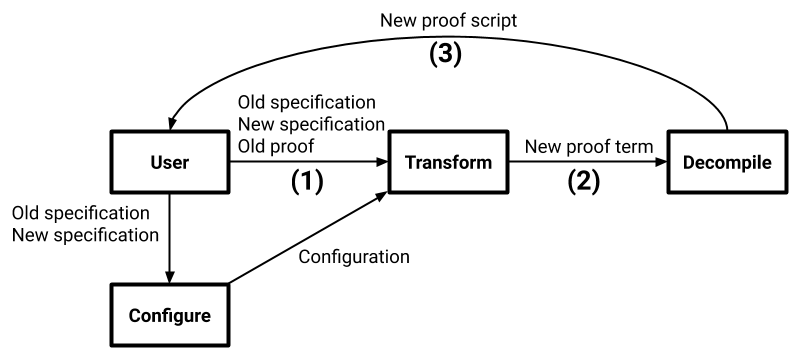
\includegraphics[width=\linewidth]{workflowa.png}
\end{minipage}
\hfill
\begin{minipage}{0.49\textwidth}
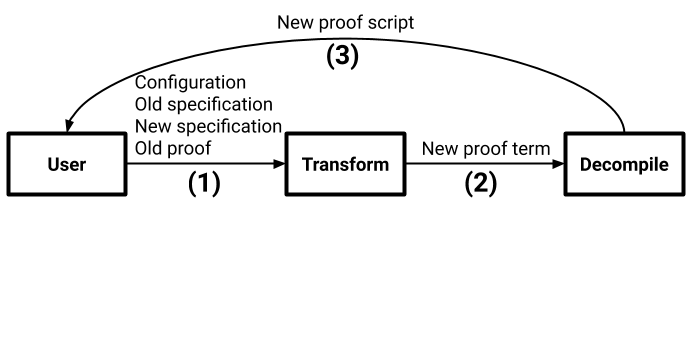
\includegraphics[width=\linewidth]{workflowb.png}
\end{minipage}
\caption{The two possible workflows for \toolname, using either automatic (left) or manual (right) configuration.}
\label{fig:system}
\end{figure}

\toolname is a tool for proof repair that is available on Github.\footnote{Link withheld for double-blind review.}
It is made of three parts:

\begin{enumerate}
\item A configurable program transformation over proof terms
\item Search procedures to configure the program transformation % TODO optionally skip, let user provide
\item A decompiler from proof terms back to tactics
\end{enumerate}
Figure~\ref{fig:system} shows how these three parts fit together.
When the user makes a change to a specification,
the user can either configure the program transformation herself, or she can
query a search procedure to try to configure it automatically.
Then, \toolname transforms the proof term appropriately, and finally
decompiles it back to tactics the user can actually maintain.

\begin{figure}
\begin{minipage}{0.46\textwidth}
   \lstinputlisting[firstline=1, lastline=3]{listswap.tex}
\end{minipage}
\hfill
\begin{minipage}{0.46\textwidth}
   \lstinputlisting[firstline=5, lastline=7]{listswap.tex}
\end{minipage}
\caption{The updated \lstinline{list} (right) is the old \lstinline{list} (left) with its two constructors swapped (\codediff{orange}).}
\label{fig:listswap}
\end{figure}

Consider a simple example: swapping the two constructors of a list (Figure~\ref{fig:listswap}).
Obviously, these are equivalent types, so this is in theory a simple refactoring.
In practice, this is not quite true, since we must change not only functions, but also proofs,
and those proofs are written in the tactic language Ltac.

Consider, for example, this proof from the standard library (using induction instead of pattern matching): % TODO explain

\begin{lstlisting}
Lemma rev_app_distr {A : Type} :
  forall (x y : list A), rev (x ++ y) = rev y ++ rev x.
Proof.
  induction x as [| a l IHl].
  induction y as [| a l IHl].
  simpl. auto.
  simpl. rewrite app_nil_r; auto.
  intro y. simpl.
  rewrite (IHl y). rewrite app_assoc; trivial.
Qed.
\end{lstlisting}
This proof no longer works after switching the constructors of \lstinline{list},
and it is not immediately clear how to adapt the proof based on tactics alone.
With \toolname, however, all we need to do is run this command: % TODO adapted for now

\begin{lstlisting}
Repair Coq.Init.Datatypes.list list in Coq.Init.Datatypes.rev_app_distr.
\end{lstlisting}
This gives us the following tactic proof:

\begin{lstlisting}
Proof.
  intros x y. revert y. induction x as [a l IHl|].
  - intro y0. simpl.
    rewrite (IHl y0). simpl. rewrite (app_assoc (rev y0) (rev l) (a :: [])). reflexivity.
  - intro y0. induction y0 as [a l IHl|].
    + simpl. rewrite (app_nil_r (rev l) (a :: [])). reflexivity.
    + reflexivity.
Qed.
\end{lstlisting}
It is then straightforward to tweak the output to something
that more closely matches the original:

\begin{lstlisting}
Proof.
  induction x as [a l IHl|].
  - intro y. simpl.
    rewrite (IHl y). rewrite app_assoc; trivial.
  - induction y as [a l IHl|].
    + simpl. rewrite app_nil_r; auto.
    + auto.
Qed.
\end{lstlisting}

We can do this for the entire list module all at once by running the \lstinline{Repair module}
command; the results of this are in \lstinline{Overview.v}.\footnote{Link withheld for double-blind review.}

This is of course a very simple example. Section~\ref{sec:search} shows how the same command
helps us support industrial integration with Coq, write dependently-typed functions and proofs for free,
switch between unary and binary natural numbers, and support repair examples from benchmarks
from real Coq proof engineers in the wild.



